\chapter{Preliminary Work}\label{C:preliminary}

This chapter presents the highlights of the initial work conducted on the creation of a Web service composition approach that combines a planning algorithm, for candidate creation and modification, with EC techniques, for optimising candidates according to their overall Quality of Service. In particular, two types of direct solution representations are explored in alignment with Objective 1: a tree-based representation, which is compatible with the existing Genetic Programming algorithm but may lead to service duplication problems, and a graph-based representation, which prevents duplication issues but requires a more complex evolutionary algorithm. These two approaches are discussed and compared in the following sections.


\section{Motivation and Problem Description}\label{Motivation and Problem Description}
\subsection{Motivation}\label{Motivation}

Our goal is to develop an automated approach for generating good service compositions. Often, many different service compositions can meet a user request but differ significantly in terms of QoS and semantic matchmaking quality. A motivating example of classical travel planning context is shown in Fig \ref{motivation}. The figure shows a DAG that represents a solution with four web services involved for a request $R$ as a composition tast. The inputs of the task are \{$TravelDepartureDate$, $HomeCity$, $ConferenceCity$, $TravelReturnDate$ \} and outputs are \{$BusTicket$, $FlightTicket$, $TouristMap$, $HotelReservation$ \}. This is a classic example of travel planning problem for people who seek for booking services of airplanes, buses and hotels reservation, and also generating tourist maps for the conference city.

\begin{figure}[h]
\centering
\fbox{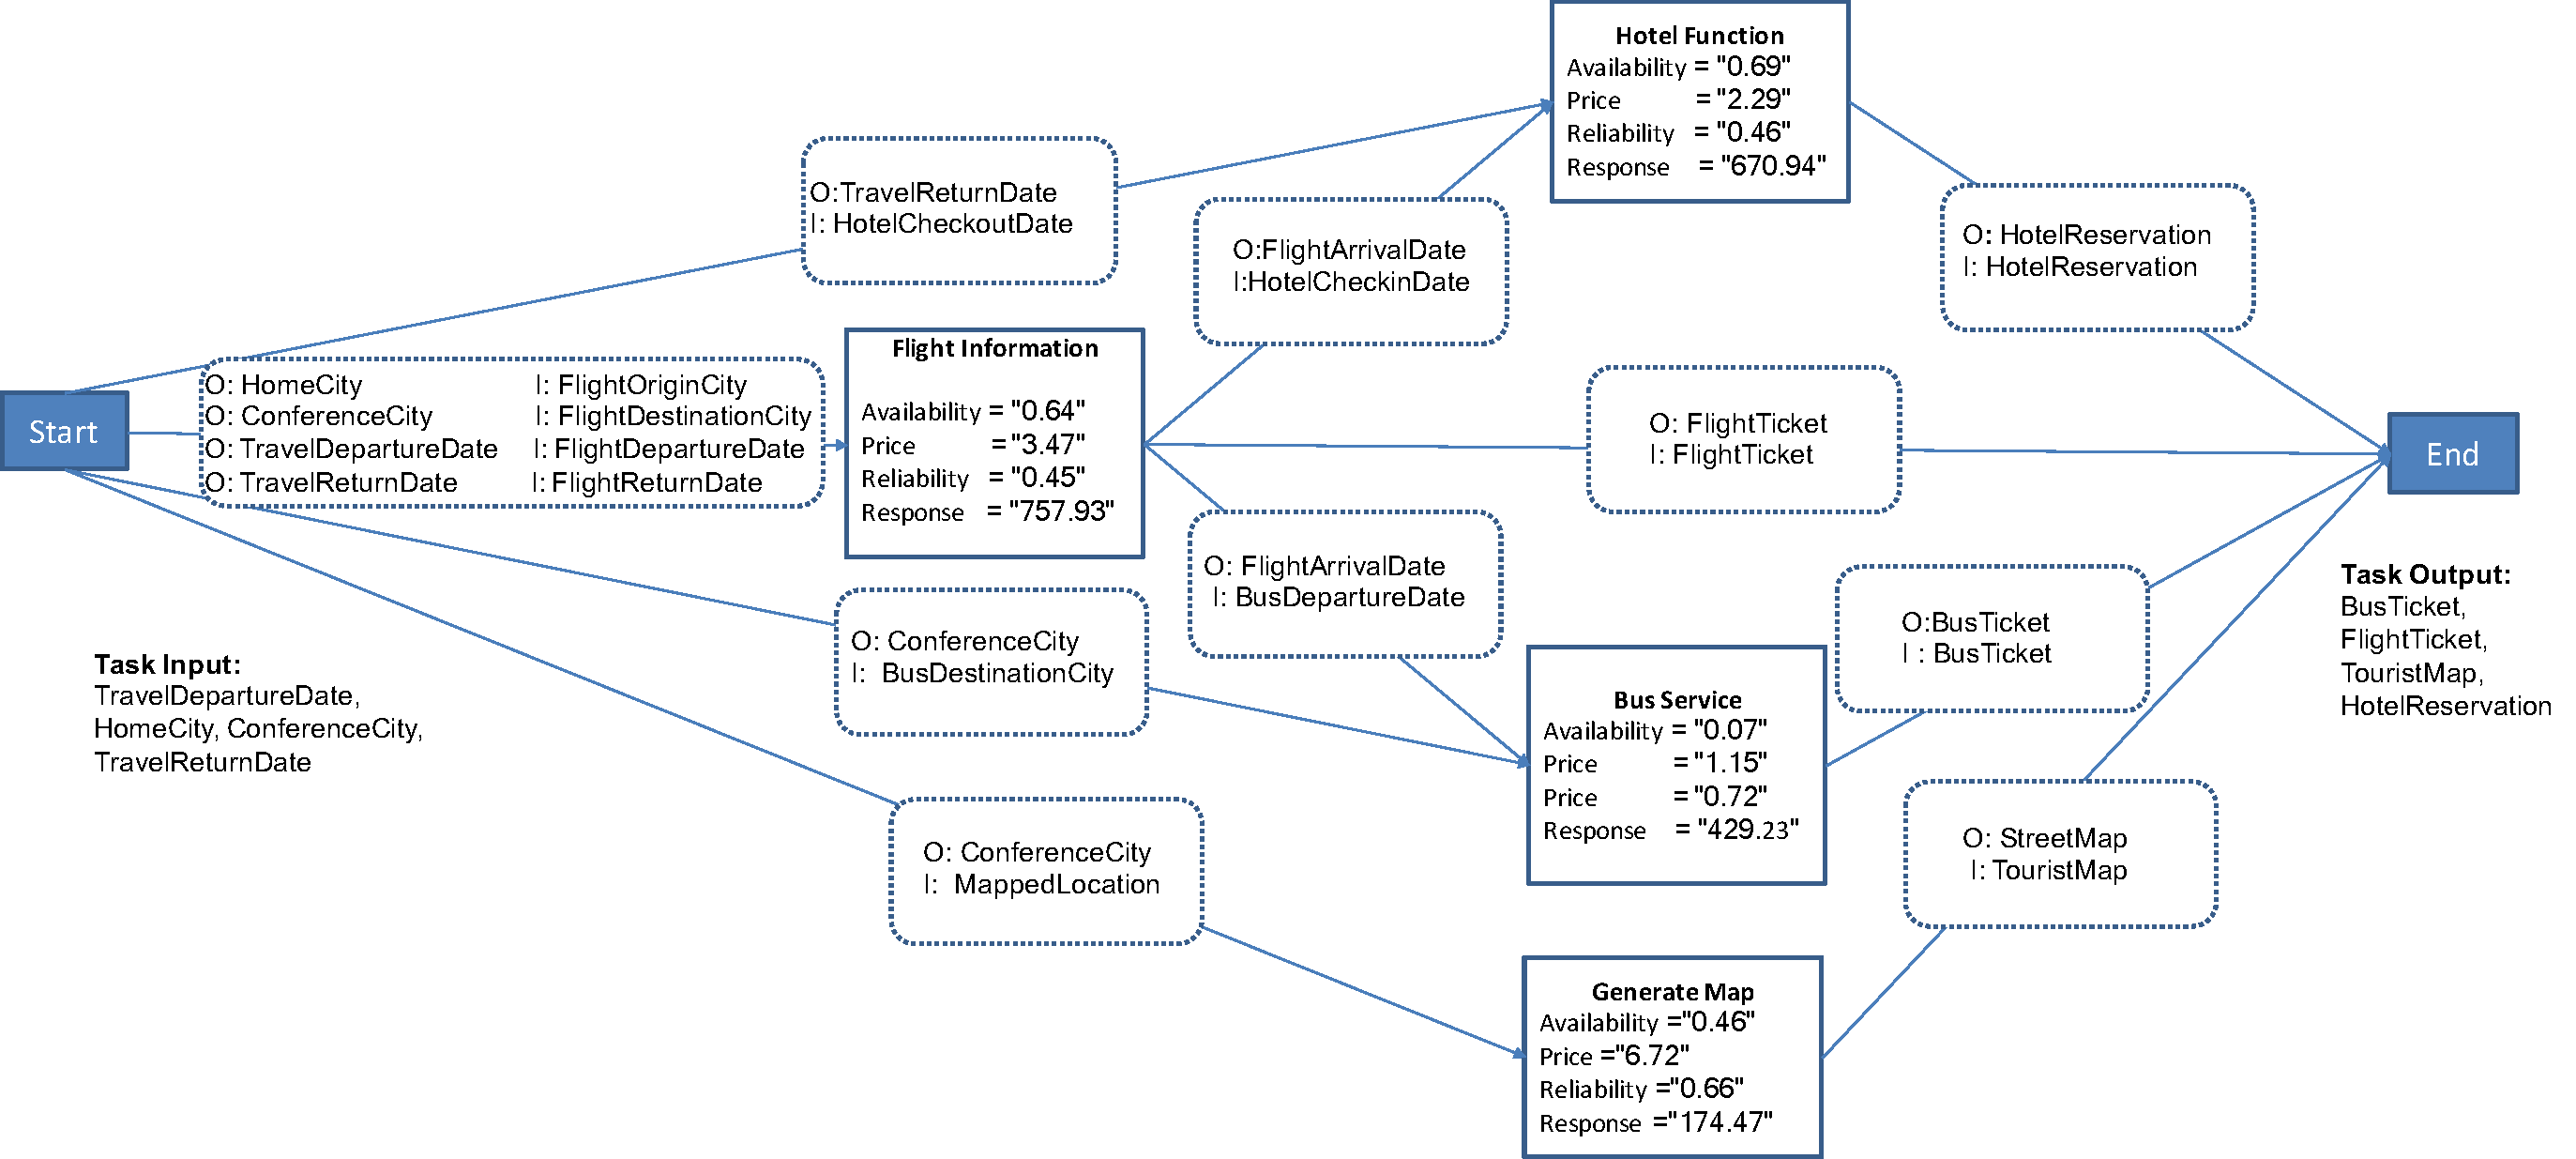
\includegraphics[scale=.25]{motivation.pdf}}
 \caption{ An example of a web service composition}
 \label{motivation}
\end{figure}

Although obtaining a correct combination of web service is essential, there are many ways to connect multiple web services chosen from a service repository. These web services provide different QoS in terms of availability, price, reliability and response time. Moreover, valid semantic matches between two connected web services could also have different matchmaking quality. For example, $Generate Map$ service produce $StreetMap$ which is considered to be a valid semantic match to $TouristMap$, while $Bus Service$ produce $BusTicket$ which is considered to be a better valid semantic match to $BusTicket$. The descriptions of these matched resources are captured in a ontology depicted in Fig .\ref{taxonomy}, where all the inputs and the outputs related to the web services are described for the travel planning problem discuss here. For example, the concept $Map$ and its sub-concept $urbanMap$ are assigned with a $touristMap$ instance and $streetMap$ instance respectively in Fig .\ref{taxonomy}. The valid semantic match is considered that an instance of $urban Map$ can be an instance of $Map$, but not vice versa. In the example of the travel planning problem, some component service must be employed to obtain a travel map. one service $GenerateMap$ can provide a street map at a price of 6.72. The other service $GenerateTouristMap$ can provide a tourist map at a price of 16.87. Because in our context a tourist map is more desirable than a street map, $GenerateTouristMap$ clearly enjoys better semantic matchmaking quality than $GenerateMap$ but will have negative impact on the QoS of the service composition (i.e., the price is much higher). One can easily imagine that similar challenges frequently occur when looking for service compositions. Hence, a good balance between QoS and semantic matchmaking quality is called for. We therefore propose a \emph{comprehensive quality model} in considering semantic matchmaking quality and QoS simultaneously.



\begin{figure}[h]
\centering
\fbox{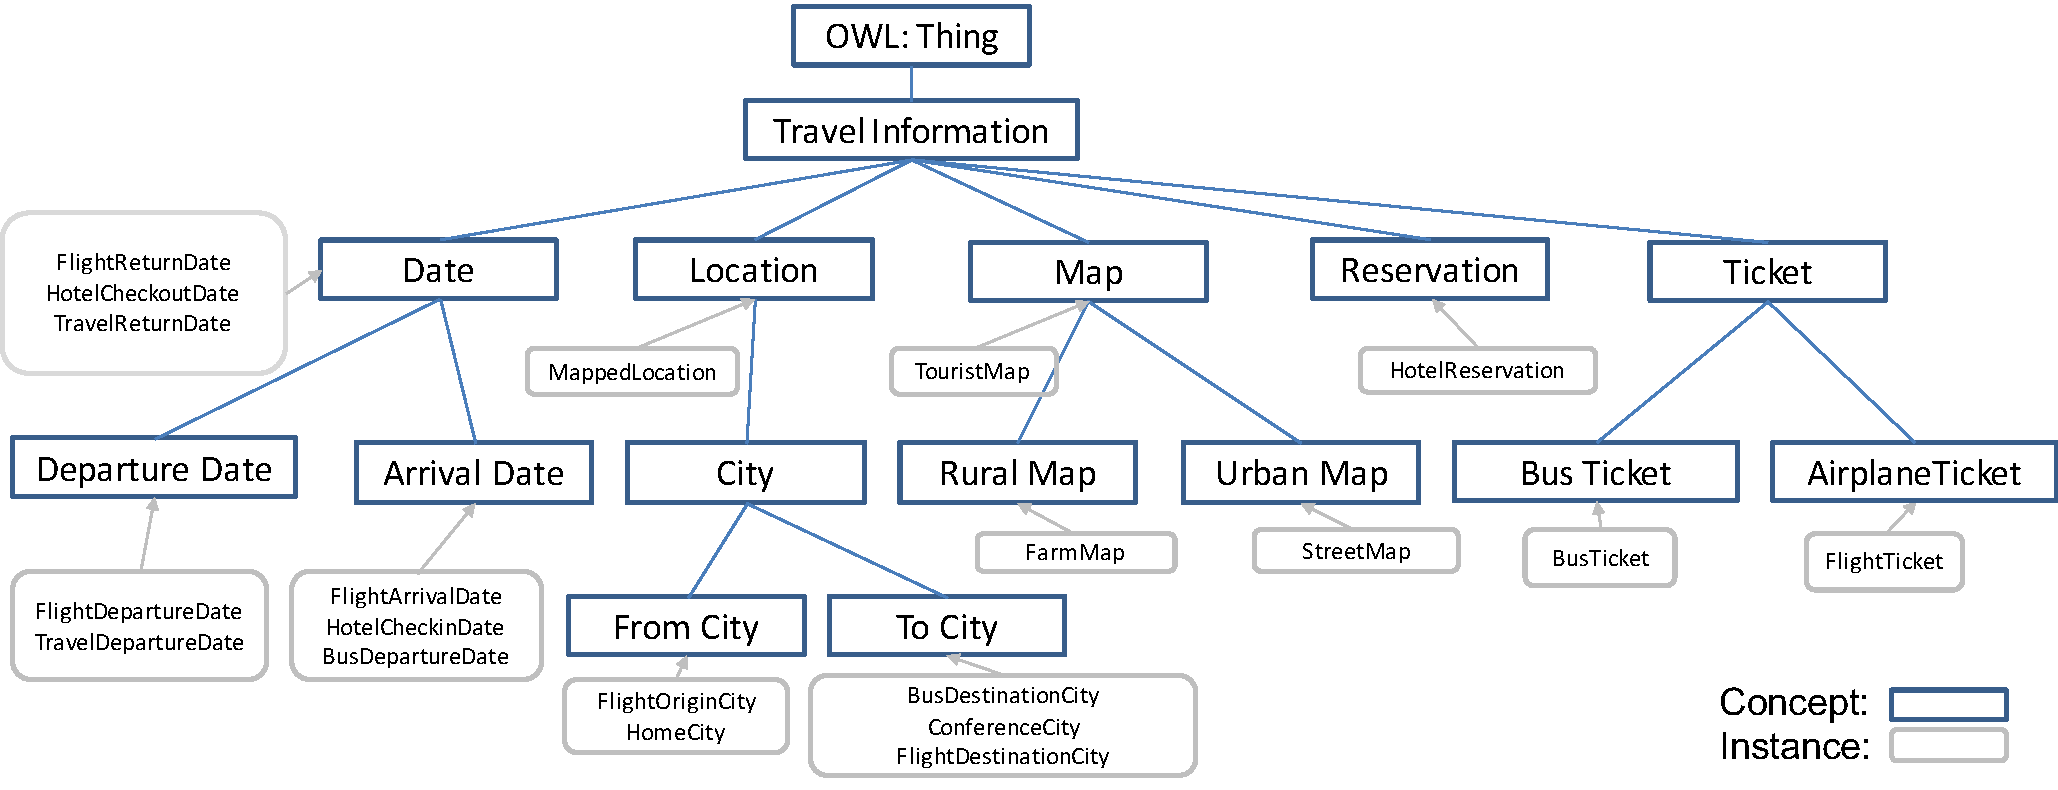
\includegraphics[scale=.28]{taxonomy.pdf}}
 \caption{ An ontology of a travel planning domain}
 \label{taxonomy}
\end{figure}



\section{Problem Description and Comprehensive Quality Model}

We consider a \emph{semantic web service} (\emph{service}, for short) as a tuple $S = (I_{S}, O_{S}, QoS_S)$ where $I_{S}$ is the set of service inputs that are consumed by $S$, $O_{S}$ the set of service outputs that are produced by $S$, and $QoS_{S}=\{t_S, c_S, r_S, a_S\}$ the set of non-functional attributes of $S$. The inputs in $I_{S}$ and outputs in $O_{S}$ are parameters that are related to concepts in an ontology $\mathcal{O}$. The attributes $t_S, c_S, r_S, a_S$ refer to the response time, cost, reliability, and availability of service $S$, respectively. These four QoS attributes are most commonly used \cite{zeng2003quality}.

A \emph{service repository} $\mathcal{SR}$ is a finite collection of services with a common ontology $\mathcal{O}$. A \emph{service request} (also called \emph{composition task}) over $\mathcal{SR}$ is a tuple $T=(I_{T}, O_{T})$ where $I_{T}$ is the set of task inputs, and $O_{T}$ the set of task outputs. The inputs in $I_{T}$ and outputs in $O_{T}$ are parameters that are related to concepts in the ontology $\mathcal{O}$.

A service composition is commonly represented as a \emph{directed acyclic graph} (DAG). It nodes correspond to the services in the composition. Two services $S$ and $S'$ are connected by an edge $e$ if some output of $S$ serves as input for $S'$. Apparently, such outputs and inputs must semantically match to ensure the correct execution of the service composition. 
The mechanism to compose services relies on the semantic descriptions of inputs and outputs, which enables inputs of services to be matched by outputs of other services. The following \emph{matchmaking types} are often used to describe the level of a match \cite{paolucci2002semantic}: For concepts $a, b$ in $\mathcal{O}$ the \emph{matchmaking} returns $exact$ if $a$ and $b$ are equivalent ($a \equiv b$), $plugin$ if $a$ is a sub-concept of $b$ ($a \sqsubseteq b$), $subsume$ if $a$ is a super-concept of $b$ ($a \sqsupseteq b$), and $fail$ if none of previous matchmaking types is returned.
In this paper we are only interested in robust compositions where only $exact$ and $plugin$ matches are considered, see \cite{lecue2009optimizing}. 

As argued in \cite{lecue2009optimizing} $plugin$ matches are less preferable than $exact$ matches due to the overheads associated with data processing. We suggest to consider the semantic similarity of concepts when comparing different $plugin$ matches. For concepts $a, b$ in $\mathcal{O}$ the \emph{semantic similarity} $sim(a, b)$ is calculated based on the edge counting method defined in Eq. (\ref{equation1}) from \cite{shet2012new}, where $N_a$, $N_b$ and $N_c$ measure the distances from concept $a$, concept $b$, and a closest common ancestor $c$ of $a$ and $b$ to the top concept of the ontology $\mathcal{O}$, respectively. 

\begin{equation}
sim(a, b){=} \frac{2N_c \cdot e^{-\lambda L/D} }{N_{a}+N_{b}}
\label{equation1}
\end{equation}
\noindent For our purposes, $\lambda$ can be set to 0 as we do not measure the similarities of neighbourhood concepts, which is not the matching type considered in this paper. 

Given a service request $T=(I_T,O_T)$, we represent a service composition solution for $T$ with services $S_1,\ldots,S_n$  by a weighted DAG, $WG=(V,E)$ with node set $V=\{Start, S_1, S_2, \ldots, S_n, End\}$ and edge set $E = \{e_{1}, e_{2},... e_{m} \}$. $Start$ and $End$ are two special services defined as $Start = (\emptyset, I_T, \emptyset )$ and $End  = (O_T, \emptyset, \emptyset)$ that account for the input and output requirements given by the request. 
%Each edge $e$ between two services $S$ and $S'$ is associated with a set of incoming outputs produced by $S$ and a set of outgoing inputs consumed by $S'$.
Each edge $e$ from a service $S$ to a service $S'$ means that service $S$ produces an output $a\in O_S$ that is matched ($exact$ or $plugin$) to an input $b\in I_{S'}$ to be consumed by service $S'$ in the composition. Based on the matchmaking type the \emph{semantic matchmaking quality} of edge $e$ can be defined as follows:
\begin{equation}
\label{equation10}
type_e = 
\begin{cases}
	1 & \text{ if $a\equiv b$ ($exact$ match)},\\
	p & \text{ if $a \sqsubseteq b$ ($plugin$ match)}
\end{cases}
\end{equation}
\begin{equation}
\label{equation11}
sim_e = sim(a,b) = \frac{2N_c}{N_{a}+N_{b}}
\end{equation}

\noindent with a suitable parameter $p, 0<p< 1$ to chosen, for discussion see Section \ref{PSO_based_approach}. However, if more than one pair of matched output and input exist from services $S$ and $S'$ respectively, $type_e$ and $sim_e$ will take on their average values.

The \emph{semantic matchmaking quality} of the service composition can be obtained by aggregating overall edges in $E$ as follows:

\begin{equation}
\label{equation6}
MT {=} \prod_{j=1}^{m} type_ {e_{j}}
\end{equation}
\begin{equation}
\label{equation7}
SIM {=} \frac{1}{m}\sum_{j=1}^m sim_ {e_{j}}
\end{equation}
The \emph{QoS} of the service composition can be obtained by aggregating the QoS values of the participating services. For a service composition with services $ S_1, S_2, ... S_n$ we obtain the reliability $R=\prod\limits^n_{k=1}r_{S_k}$, the availability $A=\prod\limits^n_{k=1}a_{S_k}$, the cost $C=\sum\limits^n_{k=1}c_{S_k}$, and the response time $T$ is the time of most time-consumption path in the composition, i.e., $$T = MAX \{\sum\limits^{\ell_j}_{k=1}t_{S_k} | \text{ $j\in\{1,\ldots,m\}$ and $\ell_j$ is the length of a path $P_j$}\}.$$

\noindent When multiple quality criteria are involved into decision making, then the overall fitness of a solution can be defined as a weighted sum of the individual criteria: 
\begin{equation}
\label{equation8}
Fitness = w_1 \hat{MT} + w_2 \hat{SIM} + w_3 \hat{A} + w_4 \hat{R} + w_5(1 - \hat{T}) + w_6(1 - \hat{C})
\end{equation}
\noindent with $\sum_{k=1}^{6} w_k= 1$. We call this objective function the \emph{comprehensive quality model} for service composition.
The weights can be adjusted according to users' preferences. Herein, the individual criteria are normalised to a range between 0 to 1, where 1 means the best value and 0 means the worst. For this purpose, we normalise $MT$, $SIM$, $A$, $R$, $T$, and $C$ so that the function value falls within the range from 0 to 1 using Eq. (\ref{equation9}). To simplify the presentation we also use the notation $(Q_1,Q_2,Q_3,Q_4,Q_5,Q_6) = (MT,SIM,A,R,T,C)$. $MT$ and $SIM$ have minimum value 0 and maximum value 1. The minimum and maximum value of $A$, $R$, $T$, and $C$ are calculated across all task-related candidates in the service repository $\mathcal{SR}$ using greedy search, for details see Section \ref{PSO_based_approach}.

\begin{equation}
\label{equation9}
\hat{Q_k} = 
\begin{cases}
	\frac{Q_k - Q_{k, min}}{Q_{k, max} - Q_{k, min}} & \text{ if $k=1,\ldots,4$ and }Q_{k, max} - Q_{k, min} \neq 0,\\
	\frac{Q_{k,max} - Q_k}{Q_{k, max} - Q_{k, min}} & \text{ if $k=5,6$ and }Q_{k, max} - Q_{k, min} \neq 0,\\
	1 & \text{ otherwise}.
\end{cases}
\end{equation}

\noindent To solve the composition task best possible the goal is to find the maximum value of the objective function in Eq. (\ref{equation8}).


\section{PSO-based Approach}\label{qswsc_approach}
\subsection{An Overview of our PSO-based Approach}\label{PSO_based_approach}

As PSO has shown promise in solving combinatorial optimisation problems, we propose a PSO-based approach to comprehensive quality-aware automated semantic web service composition. Fig. \ref{overview} shows an overview of our approach consisting of four steps: 
\begin{figure}[h]
\centering
\fbox{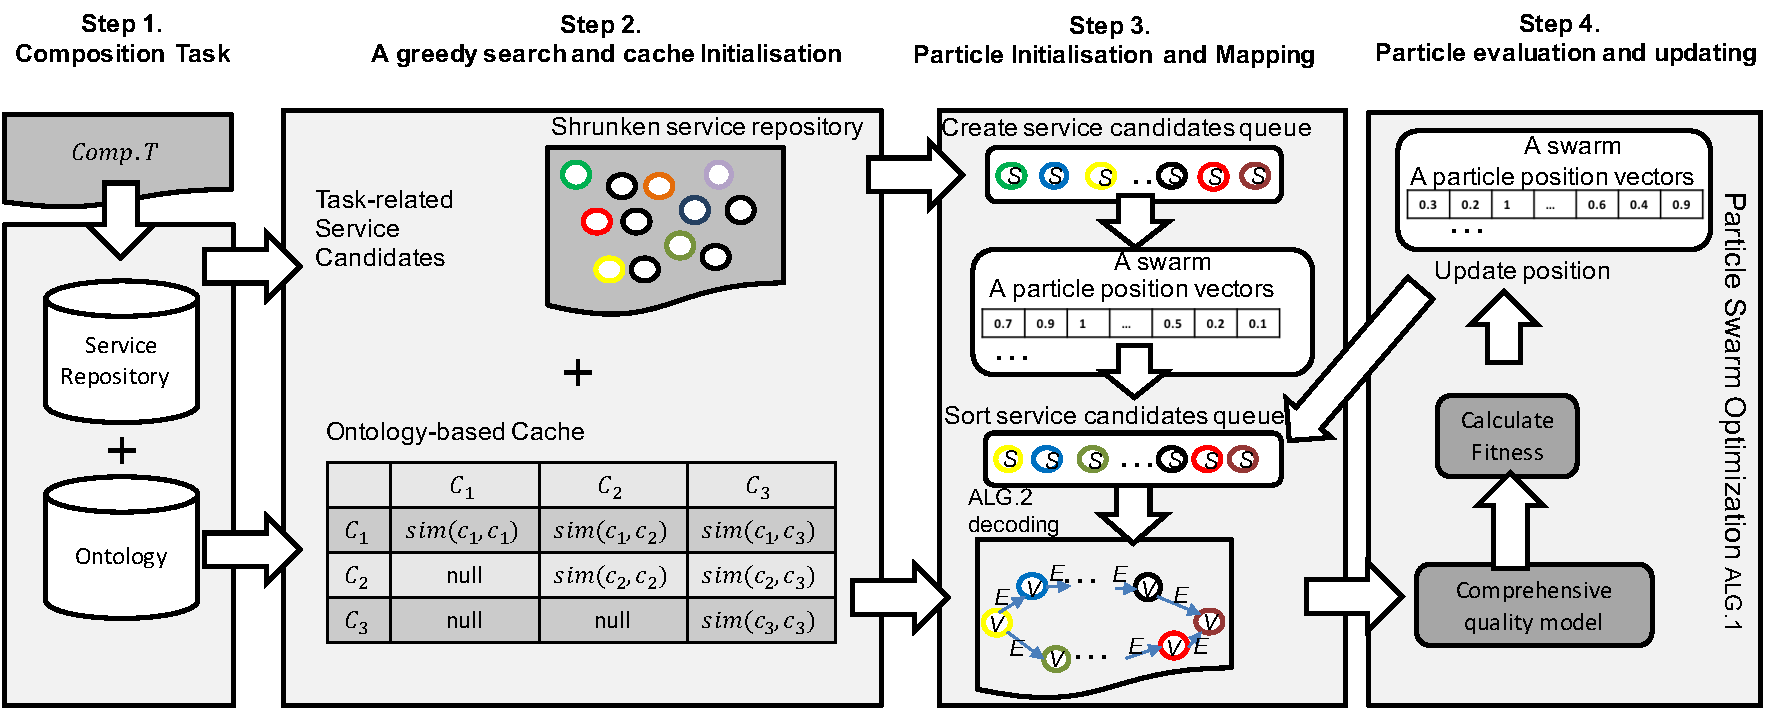
\includegraphics[scale=.5]{overview.pdf}}
 \caption{An overview of our PSO-based approach to comprehensive quality-aware automated semantic web service composition.}
 \label{overview}
\end{figure}

Step 1: The composition process is triggered by a composition task, which is clearly defined in Section \ref{problemDes}. 

Step 2: The composition task is used to discover all task-related service candidates using a greedy search algorithm adopted from \cite{ma2015hybrid}, which contributes to a shrunken service repository. This greedy search algorithm keeps adding outputs of the invoked services as available outputs (initialised with $I_{T}$) , and these available outputs are used to discover task-related services from a service repository and updated with the outputs of these discovered services. This operation is repeated until no service is satisfied by the available outputs. During the greedy search, an ontology-based cache ($cache$) is initialised, which stores the concept similarities of matched inputs and outputs of task-related candidates. This $cache$ is also used to discover services by checking whether $null$ is returned by given two output-related and input-related concepts.

Step 3 and Step 4: These two steps follow the standard PSO steps \cite{shi2001particle} except for some differences in particles mapping and decoding processes. In particular, these two differences are related to sorting a created service queue using service-to-index mapping for a particle' position vectors and evaluating the fitness of a particle after decoding this service queue into a $WG$ respectively. Those differences are further addressed in Algorithms \ref{novelSteps} and \ref{graph_building} in Section \ref{POS-based_algomargin}.



\subsection{The Algorithms for our PSO-based Approach}\label{POS-based_algomargin}
The overall algorithm investigated here is made up of a PSO-based web service composition technique (Algorithm \ref{novelSteps}) and a $WG$ creating technique from a service queue (Algorithm \ref{graph_building}). In Algorithm \ref{novelSteps}, the  steps $4$, $5$, $6$ and $7$ are different from those of standard PSO: In step 4, the size of task-related service candidates generated by a greedy search determines the size of each particle's position. Each service candidate in a created service candidates queue is mapped to an index of a particle’s position vectors, where each vector has a weight value between 0.0 and 1.0. In step 5, service candidates in the queue are sorted according to their corresponding weight values in descending order. In step 6, this sorted queue is used as one of the inputs of the forward decoding Algorithm \ref{graph_building} to create a $WG$. In step 7, the fitness value of the created $WG$ is the fitness value of the particle calculated by the comprehensive model discussed in Section \ref{Comprehensive_Quality_Model}.
\begin{algorithm}
 %\LinesNumbered
 \SetKwInOut{Input}{Input}\SetKwInOut{Output}{Output}
 \SetKwFunction{generateWeightedGraph}{generateWeightedGraph}
 \SetKwProg{Procedure}{Procedure}{}{}
 \SetNlSty{}{}{:}
 Randomly initialise each particle in the swarm\;
  \While {max. iterations not met}{
     \ForEach{particle in the swarm}{
     Create a service candidates queue and map service candidates to a particle's position vectors\;
     Sort the service queue by position vectors' weights\;
     Use Algorithm \ref{graph_building} to create a $WG$ from the service queue \;
     Calculate the $WG$ fitness value\;
     
      \eIf{fitness value better than pBest}{    
        Assign current fitness as new \emph{pBest}\;
       }{
        Keep previous \emph{pBest}\;
       }	
     }
    Assign best particle's \emph{pBest} value to \emph{gBest}, if better than \emph{gBest}\;
 	Calculate the velocity of each particle\;
  	Update the position of each particle\;
  }
\caption{Steps of PSO-based service composition technique \cite{da2016particle}.}
\label{novelSteps}
\end{algorithm} 

Algorithm  \ref{graph_building} is a forward graph building algorithm extended from \cite{blum1997fast}. This algorithm takes one input, a sorted service queue from step 5 of Algorithm \ref{novelSteps}. Note that different service queues may lead to different $WGs$. In addition. $I_{T}$, $O_{T}$ and $cache$ are also taken as the inputs. Firstly, $Start$ and $End$ are added to $V$ of $WG$ as an initialisation, and $OutputSet$ is also created with $I_{T}$. The following steps are repeated until $O_{T}$ can be satisfied by $Outputset$ or the service queue is $null$. If all the inputs $I_{S}$ of the first popped  $S$ from $queue$ can be satisfied by provided outputs from $OutputSet$, this $S$ is added to $V$ and its outputs are added to $OutputSet$, and $S$ is removed from $queue$. Otherwise, the second popped  $S$ from $queue$ is considered for these operations. Meanwhile, $e$ is created with $type_e$ and $sim_e$ if $S$ is added, and calculated using information provided from $cache$. This forward graph building technique could lead to more services and edges connected to the $WG$, these redundancies should be removed before $WG$ is returned.

\begin{algorithm}
 \SetKwInOut{Input}{Input}\SetKwInOut{Output}{Output}
 \SetKwFunction{createWeightedDAG}{createWeightedDAG}
 \SetKwProg{Procedure}{Procedure}{}{}
 %\LinesNumbered
 \SetNlSty{}{}{:}
 % \Procedure{}{
 \Input{ $I_T$, $O_T$, $queue$, $cache$}
 \Output{WG}
 $WG = (V, E)$\;
 $V \leftarrow$ \{$Start$, $End$ \} \;
 $OutputSet \leftarrow$ \{$I_{T}$\}\;
  \While { $O_{T}$ not satisfied by $OutputSet$}{
     \ForEach{$S$ in $queue$}{
      \uIf{$I_{S}$ satisfied by $OutputSet$}{  
        insert $S$ into $V$ \;  
        adjoin $O_{S}$ to $OutputSet$\;
        $queue$.remove $S$\;   
        $e \leftarrow$ calculate $type_e$, $sim_e$ using $cache$\;
        insert $e$ into $E$\;
       }	
     }
  }
 remove $dangling$ $nodes$ and $edges$ from $WG$\; 
 \KwRet $WG$\;
 %}
 \caption{Create a $WG$ from a sorted service queue.}
\label{graph_building}
\end{algorithm} 


\subsection{Ontology-based Cached Optimisation} \label{indexCache}
In GP, the tree structure representation, which is converted from weighted graphs with edges as the quality of semantic matchmaking and node with QoS. The bottlenecks of our whole approach lie in building weighted graph for initialisation and mutation. In particularly, it refers the size of service repository and cost of semantic matchmaking quality calculation. The size of service of repository could be shrunken into the task-related web services using greedy search. Later on, the cost of semantic quality calculation could be pre-calculated for parameter-related concepts from the task-related webs services. The key idea of the index is to create a map using a pair of keys, output-related concepts and potentially matched input-related concepts with considering different levels of match types, and the map values store $mt_{p}$ and $mt_{s}$. This optimised cache also contributes to less and constant time for weighted graph building for initialisation and mutation.



\subsection{Genetic Programming Overview}\label{problem}

GP \cite{koza1992genetic} is an automated technique for producing and searching computer programs in a solution space, which is considered as a particular application of Genetic Algorithm with a set of different encoded genes.  In GP, each individual as a chromosome, which is commonly represented as a tree structure, refers to a candidate solution in a population. The tree structure has a terminal set and a function set, where variables, constants and functions are consisted of respectively. Also,  the tree structure is considered be efficiently traversed and evaluated.

Nature evolution and selection of individual in a population are automated simulated in GP \cite{koza1992genetic}. A fitness function is utilised to evaluate the degree of how good (or bad) of each individual after it is evolved. Once all individuals within one generation are all evaluated, three genetic operators consisting of reproduction, crossover, and mutation are involved in to generate next generation. Reproduction operator retains the elite individual without any changes. Crossover operator replaces one node of one individual with another node of another individual. Mutation operator replaces a randomly selected node in an individual. The whole evaluation process will continue until an optimised solution found or a pre-defined number of generation reached. Therefore, We identify the set of terminals, the set of functions, the fitness function and other relevant parameters to perform a GP-based algorithm.

This chapter presents the highlights of the initial work conducted on the creation of a Web service composition approach that combines a planning algorithm, for candidate creation and modification, with EC techniques, for optimising candidates according to their overall Quality of Service. In particular, two types of direct solution representations are explored, in alignment with Objective \ref{obj:rep}: a \textit{tree-based representation}, which is compatible with the existing Genetic Programming algorithm but may lead to service duplication problems, and a \textit{graph-based representation}, which prevents duplication issues but requires a more complex evolutionary algorithm. These two approaches are discussed and compared in the following sections.



\subsection{Ontology-based Index Cached Optimisation}\label{indexCache}
our PSO-based approach demands decoding processes from optimised queues to weighted DAGs, a bottleneck of efficiently constructing weighted DAGs lie in building required information of edges, which is related to the cost of $fullmatch$
$(a \Rightarrow b)$ identifications and $sim(a, b)$ calculations between input-related and output-related concepts of service candidates. To efficiently construct weighted DAGs, we calculate $sim(a, b)$ of all $fullmatch(a \Rightarrow b)$ interleaving with the greedy search discussed in Sect \ref{PSO_based_approach}. This information is stored in a table structure with special $X$ value if no $fullmatch(a \Rightarrow b)$ is satisfied. Therefore, this optimised cache contributes to less and constant time for weighted DAG building through the evolutionary process.

\section{Experiment Design}\label{experiment_design}
In this section, we employ a quantitative evaluation approach with a benchmark dataset used in \cite{ma2015hybrid,da2016genetic}, which is an augmented version of Web Service Challenge 2009 (WSC09) including QoS attributes. This benchmark dataset contains five tasks with variable numbers of services, and ontologies, which is considered as a challenge dataset for measuring the scalability of our quality evaluation model. Table \ref{wsc09datasetTable} presents the features of the WSC’09 dataset. The number of concepts, individuals in the ontology and services in each data set is shown in the second, third, fourth column respectively. Also, we extend all the datasets with QoS attributes from service providers to enable our evaluation.  Two objectives of this evaluation are to: $(1)$ evaluate the effectiveness of our PSO-based approach, see comparison test in Section \ref{comparisonTestWithGP}.
$(2)$ evaluate the effectiveness of our proposed comprehensive quality model to achieve a desirable balance on semantic matchmaking quality and QoS, see comparison test in Section \ref{comparisonTest}.

\begin{table}[]
\centering
\caption{Features of the WSC09 datasets}
\label{wsc09datasetTable}
\begin{tabular}{l|l|l|l}
\hline
\multicolumn{1}{c|}{Dataset} & No.Concept & No.Individual & No.Service \\ \hline
WSC09 01                     & 1578       &3102           &572      \\ \hline
WSC09 02                     & 12388      &24815          &4129      \\ \hline
WSC09 03                     & 18573      &37316          &8138      \\ \hline
WSC09 04                     & 18673      &37324          &8301      \\ \hline
WSC09 05                     & 31044      &62132          &15211    \\ \hline
\end{tabular}
\end{table}


The parameters for the PSO are chosen from the settings from \cite{shi2001particle}, In particular, PSO population size is 30 with 100 generations. We run 30 times independently for each dataset. We configure the weights of fitness function to properly balance semantic matchmaking quality and QoS. Therefore, $w_{1}$ and $w_{2}$ are set equally to 0.25, and $w_{3}$, $w_{4}$, $w_{5}$, $w_{6}$ are all set to 0.125. The $p$ of $type_e$ is set to 0.75 ($plugin$ match) according to \cite{lecue2009optimizing}. In general, weight settings and parameter $p$ are decided by users' preferences.
\vspace{-0.5cm}

\section{Experiment Results}\label{experiment_results}


\subsection{Comparison Test for GP-based vs. PSO-based approach}\label{comparisonTestWithGP}
To evaluate the effectiveness of our proposed PSO-based approach, we compare our PSO-based method with one recent GP-based approach \cite{ma2015hybrid} using our proposed comprehensive quality model. We extend this GP-based approach by measuring the semantic matchmaking quality between parent nodes and children nodes. To make a fair comparison, we use the same number of evaluations (3000 times) for these two approach. We set the parameters of that GP-based approach as 30 individuals and 100 generations, which is considered to be proper settings referring to \cite{da2015gp}.

The first column of Table \ref{meanFitness} shows five tasks from WSC09. The second and third column of Table \ref{meanFitness} show the original service repository size and the shrunk service repository size after the greedy search respectively regarding the five tasks. This greedy search helps reducing the original repository size significantly, which contributes to a reduced searching space. The fourth and fifth column of Table \ref{meanFitness} show the mean fitness values of 30 independent runs accomplished by two methods. We employ independent-samples T tests to test the significant differences in mean fitness value. The results show that the PSO-based approach outperforms the existing GP-based approach in most cases except Task 3. Note that all $p$-values are consistently smaller than 0.01. Using our PSO-based approach, small changes to sorted queues (particles in PSO) could lead to big changes to the composition solutions. This enables the PSO-based approach to escape from local optima more easily than the GP-based approach. 
%the PSO-based approach performs significantly better than the GP-based approach in finding optimal solutions. It may be that the GP-based approach is stuck in local optima in a very large search space due to its evolutionary operators. On the other hand, the decoding process used by the PSO-based approach allows for small changes that more effectively prevent this from happening.

\begin{table}[]
\centering
\caption{Mean fitness values for comparing GP-based approach}
\label{meanFitness}
\begin{tabular}{c|c|c|l|l}
\hline
\multicolumn{1}{c|}{WSC09} &Original $\mathcal{SR}$  &Shrunken $\mathcal{SR}$   &PSO-based approach & GP-based approach  \\ \hline
Task 1                     &572            &80    &0.5592 $\pm$ 0.0128  $\uparrow$  &0.5207 $\pm$ 0.0208           \\ \hline
Task 2                     &4129           &140   &0.4701 $\pm$ 0.0011  $\uparrow$  &0.4597 $\pm$ 0.0029          \\ \hline
Task 3                     &8138           &153   &0.5504 $\pm$ 0.0128              &0.5679 $\pm$ 0.0234 $\uparrow$   \\ \hline
Task 4                     &8301           &330   &0.4690 $\pm$ 0.0017  $\uparrow$  &0.4317 $\pm$ 0.0097            \\ \hline
Task 5                     &15211          &237   &0.4694 $\pm$ 0.0008  $\uparrow$  &0.2452 $\pm$ 0.0369            \\ \hline
\end{tabular}
\end{table}


\subsection{Comparison Test for Comprehensive Quality Model vs. QoS Model}\label{comparisonTest}

Recently, a QoS Model, $Fitness = w_1 \hat{A} + w_2 \hat{R} + w_3(1 - \hat{T}) + w_4(1 - \hat{C})$, where $\sum_{i=1}^{4} w_i = 1$, is widely used for QoS-aware web service composition \cite{ma2015hybrid,da2016particle,da2015graphevol}. To show the effectiveness of our proposed comprehensive quality model, we compare the best solutions found by this QoS model and our comprehensive model using our PSO-based approach. We record and compare the mean values of both $SM$ ($SM = 0.5 \hat{MT} + 0.5 \hat{SIM}$) and $QoS$($QoS = 0.25 \hat{A} + 0.25 \hat{R} + 0.25(1 - \hat{T}) + 0.25(1 - \hat{C})$) of best solutions over 30 independent runs. To make the comparison informative, all these recorded values have been normalised from 0 to 1, and compared using independent-samples t tests, see Table \ref{decisionTable}. 

We observe an interesting pattern from Table \ref{decisionTable}. The mean values of $QoS$ using QoS model are significantly higher than those using comprehensive quality model for Tasks 2, 3, 4 and 5. However, the mean value of $SM$ using the comprehensive quality model are significantly higher than those using the QoS model, while a slight trade-off in $QoS$ are observed in all tasks. In addition, our comprehensive model achieves a consistently higher comprehensive quality in terms of a combination of $SM$ and $QoS$, which is significantly better in Tasks 1, 2, 3 and 4. 

\begin{table}[]
\footnotesize
\centering
\caption{Mean values of $SM$, $QoS$ and sum of $SM$ and $QoS$ for QoS model and comprehensive quality model using PSO-based approach}
\label{decisionTable}
\begin{tabular}{c|c|l|l}
\hline
\multicolumn{2}{c|}{WSC09}              & \shortstack{QoS \\ Model}         &\shortstack{Comprehensive Quality \\ Model} \\ \hline
\multirow{3}{*}{Task1}  &$SM$      &0.5373 $\pm$ 0.0267               &0.5580 $\pm$ 0.0094 $\uparrow$ \\ \cline{2-4}
                        &$QoS$     &0.5574 $\pm$ 0.0156               &0.5604 $\pm$ 0.0164            \\ \cline{2-4}
                        &$SM+QoS$  &1.0947 $\pm$ 0.0423               &1.1184 $\pm$ 0.0258 $\uparrow$ \\ \hline
\multirow{3}{*}{Task2}  &$SM$      &0.4549 $\pm$ 0.0033               &0.4630 $\pm$ 0.0042 $\uparrow$ \\ \cline{2-4} 
                        &$QoS$     &0.4800 $\pm$ 0.0012 $\uparrow$    &0.4772 $\pm$ 0.0025            \\ \cline{2-4}
                        &$SM+QoS$  &0.9349 $\pm$ 0.0045               &0.9402 $\pm$ 0.0067 $\uparrow$           \\ \hline
\multirow{3}{*}{Task3}  &$SM$      &0.5538 $\pm$ 0.0082               &0.6093 $\pm$ 0.0054 $\uparrow$ \\ \cline{2-4} 
                        &$QoS$     &0.4940 $\pm$ 0.0013 $\uparrow$    &0.4913 $\pm$ 0.0009            \\ \cline{2-4}
                        &$SM+QoS$  &1.0478 $\pm$ 0.0095               &1.1006 $\pm$ 0.0063 $\uparrow$           \\ \hline
\multirow{3}{*}{Task4}  &$SM$      &0.4398 $\pm$ 0.0037               &0.4604 $\pm$ 0.0000 $\uparrow$ \\ \cline{2-4} 
                        &$QoS$     &0.4845 $\pm$ 0.0010 $\uparrow$    &0.4734 $\pm$ 0.0044            \\ \cline{2-4}
                        &$SM+QoS$  &0.9243 $\pm$ 0.0047               &0.9338 $\pm$ 0.0044 $\uparrow$           \\ \hline
\multirow{3}{*}{Task5}  &$SM$      &0.4580 $\pm$ 0.0065               &0.4639 $\pm$ 0.0013 $\uparrow$ \\ \cline{2-4} 
                        &$QoS$     &0.4764 $\pm$ 0.0005 $\uparrow$    &0.4750 $\pm$ 0.0007            \\ \cline{2-4}
                        &$SM+QoS$  &0.9344 $\pm$ 0.0070               &0.9389 $\pm$ 0.0020           \\ \hline
\end{tabular}
\end{table}

\subsection{Further Discussion}\label{discuss1}
To analyse the effectiveness of achieving a good comprehensive quality at the expense of slightly reduced QoS, we demonstrate two best solutions produced using Task 3 as an example. Fig. \ref{comparisontest} $(1)$ and $(2)$ show two weighted DAGs $WG_1$ and $WG_2$ that have been obtained as the best service compositions solutions based on the QoS model and on the comprehensive quality model, respectively. Both $WGs$ have exactly the same service workflow structure, but some service vertices and edges denoted in red are different. To better understand these differences, we list the overall semantic matchmaking quality $SM$,  overall $QoS$ and semantic matchmaking quality associated to these different edges in $WG_1$ and $WG_2$. (Note: $sm_{e_n} = 0.5type_{e_n} + 0.5 sim_{e_n}$), where $\Delta Q$ reveals the gain (positive $\Delta Q$) or a loss (negative $\Delta Q$) of the listed qualities for our comprehensive quality model. Therefore, we achieve a comprehensive quality gain of 0.1433, which is the result of a gain in semantic matchmaking quality (+0.1467) and a loss in $QoS$ (-0.0034). To understand the improvement of semantic matchmaking quality from these numbers, we pick up $e_4$ that is associated with the smallest $\Delta Q$. The $e_4$ of $WG_1$ and $WG_2$ has two different source nodes, $Ser1640238160$ and $Ser947554374$, and two the same end nodes. $Ser1640238160$ and $Ser947554374$ are services with output parameters $Inst582785907$ and  $Inst795998200$ corresponds to two concepts $Con2037585750$ and $Con103314376$ respectively in the given ontology shown in Fig. \ref{comparisontest} $(4)$. As $Inst658772240$ is a required parameter of $End$, and related to concept $Con2113572083$, $Inst795998200$ is closer to the required output $Inst658772240$ than $Inst582785907$. Therefore,  $Ser947554374$ is selected with a better semantic matchmaking quality compared to $Ser1640238160$.

\begin{figure}[h]
\centering{
\fbox{
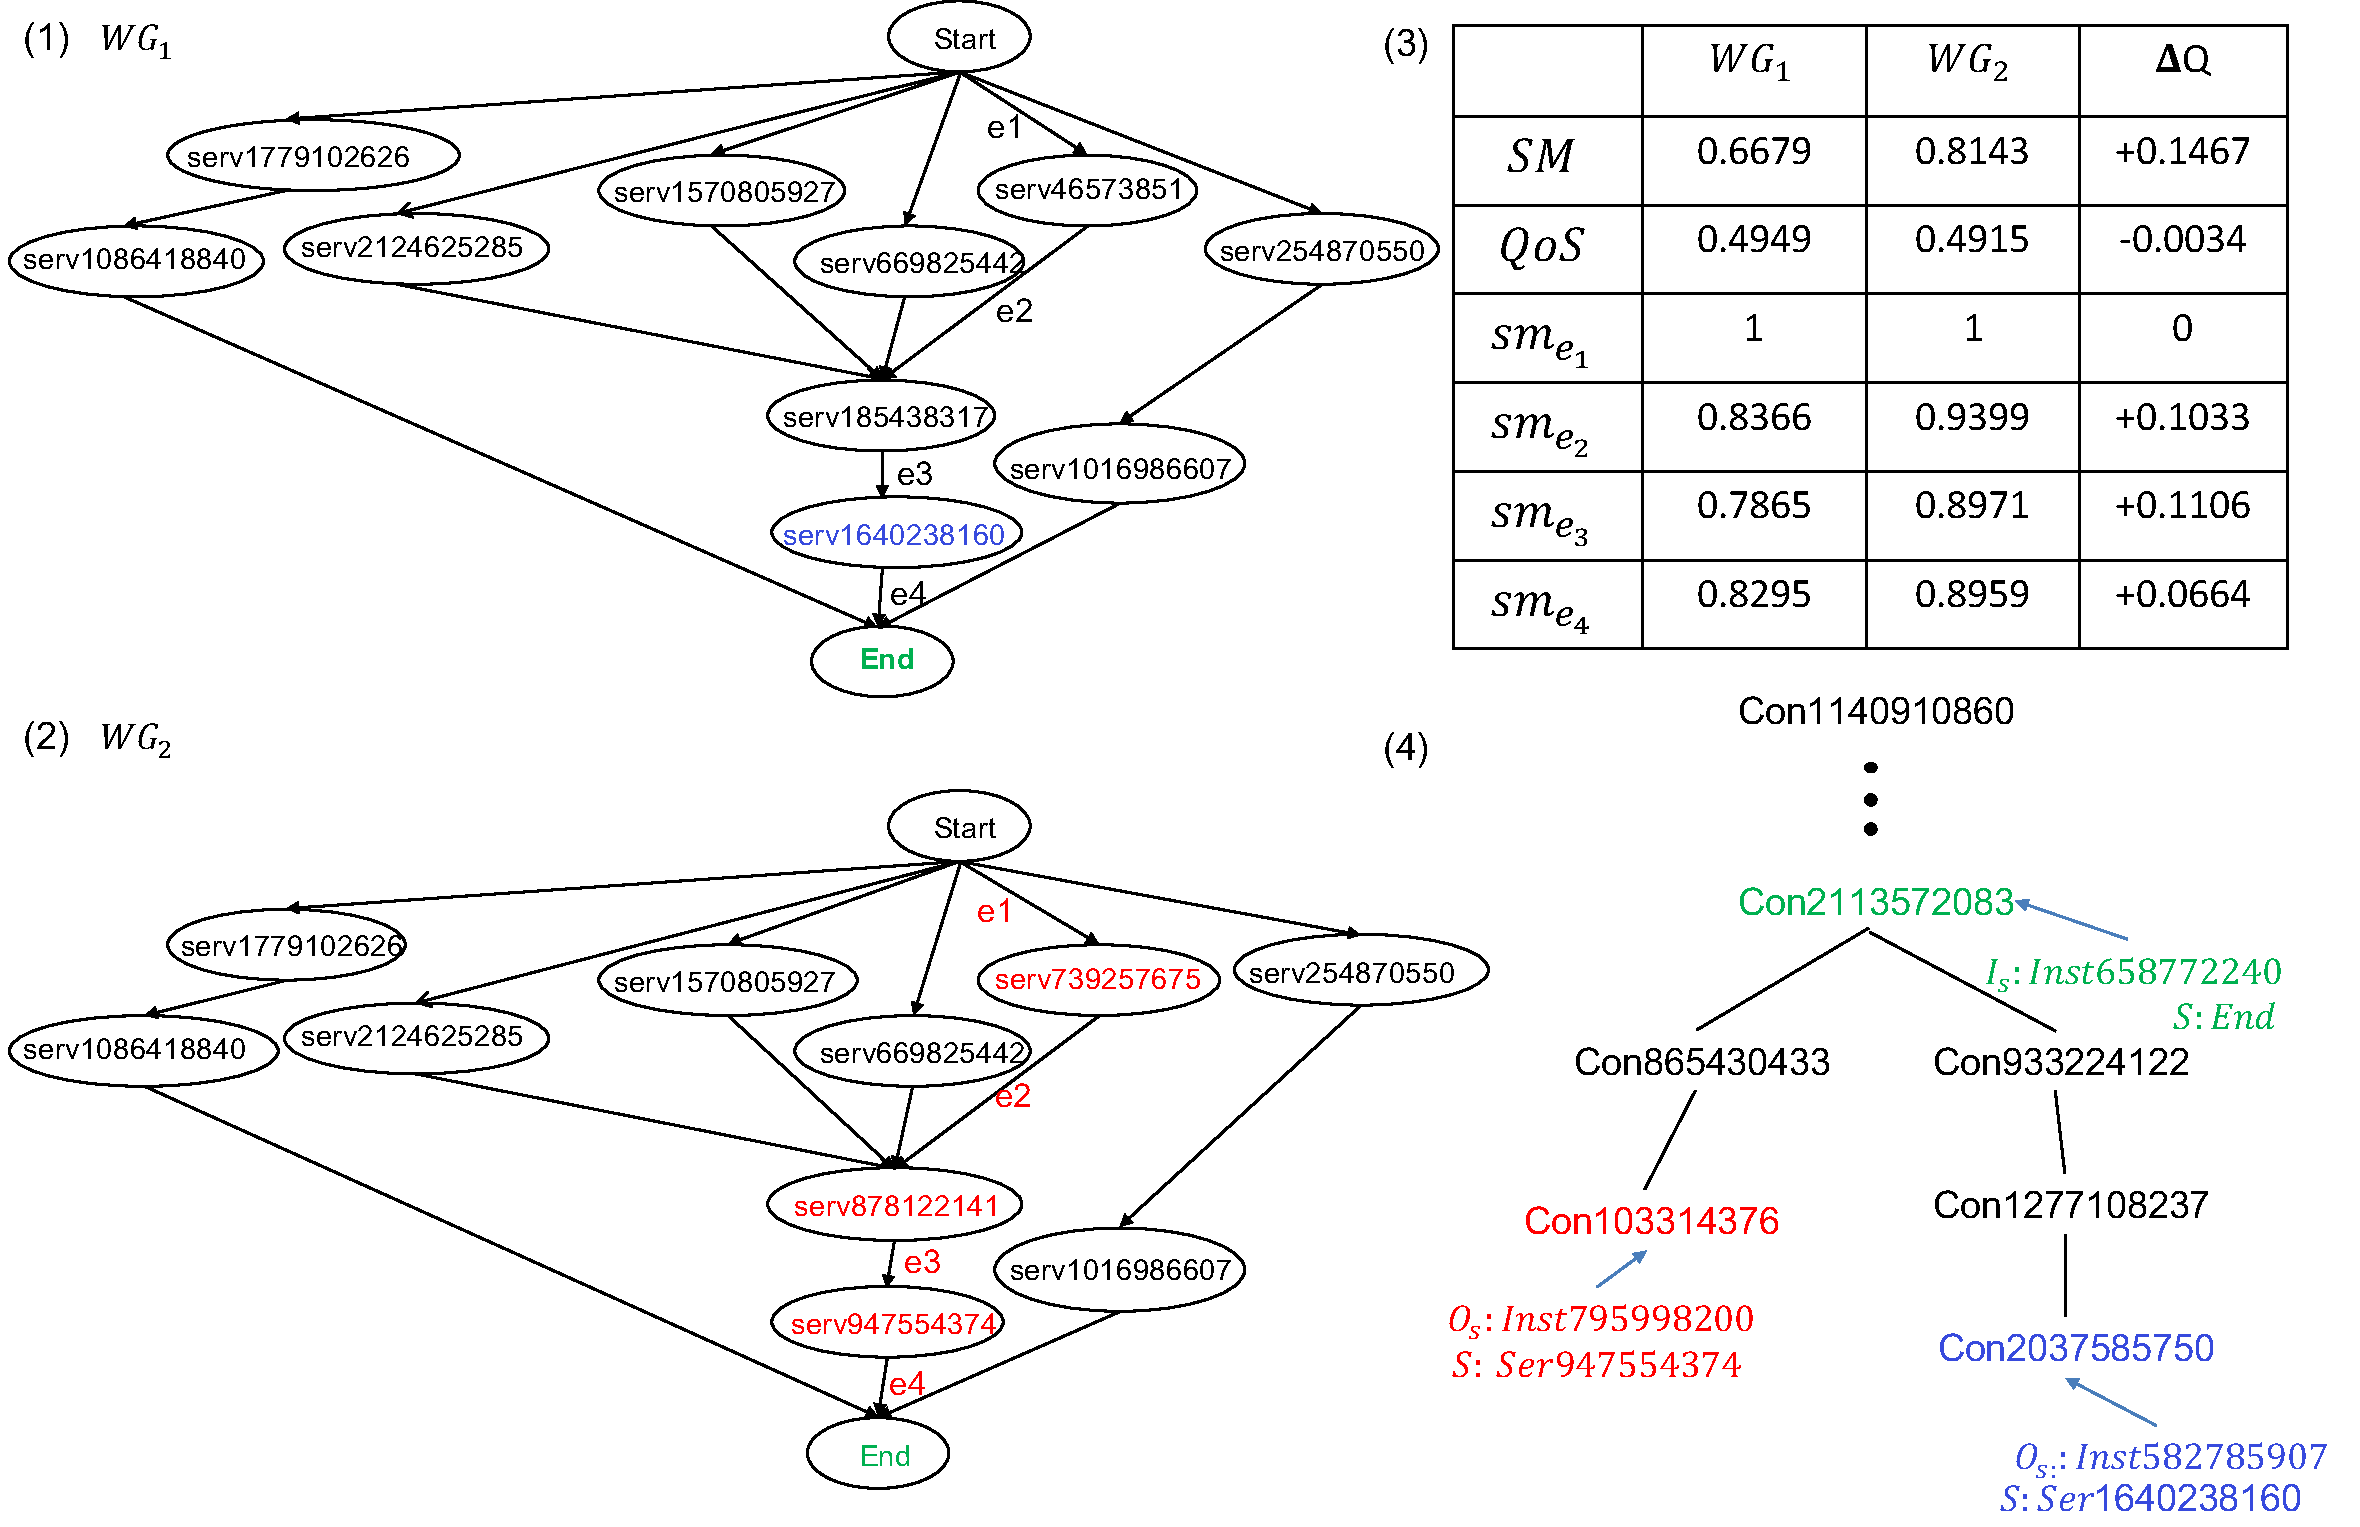
\includegraphics[scale=.29]{comparisontest.pdf}}}
 \caption{An example for the comparison of the best solutions obtained based on the QoS model and on the comprehensive quality model for Task 3.}
 \label{comparisontest}
\end{figure}





The modified main algorithm $toTree()$ in Algorithm \ref{toTree} consisting of two stages: $cN$ is located at $Start$ and $cN$ isn't located at $start$. In the first stage, two cases are considered according to the size of $cN$'s outgoing edges. If the size equals 1 (line 3-4), a sequence node is created with a specific $Start$ service node as a right child, and a returned node of $getNextNode()$ (line 26) as a left child. Otherwise(line 5-6), a same sequence node is created with a different left child, a returned node of $parallelNode()$ (line 38). In the second stage, there are two cases (line 13-18 and line 19-24) are involved in according to the size of $cN$'s outgoing edges without considering those target $End$. Each case are considered under two conditions (line 14 and 20) that there exists one outgoing edge of $cN$ targets $End$ or not. Therefore, same sequence nodes discussed in the first stage are created with different service node $cN$ as a right child, rather than $Start$. If the opposite condition  (line 16 and 22) holds, those sequence nodes in the first condition are wrapped as right child of a $parallelNode$, whose left child is a sequence node with a $cN$ service node as its left child and a $End$ service node as right child. We also present the functions for creating sequence node: $seqNode()$ and creating parallel nodes: $parallelNode()$ in Algorithm \ref{toTree}.
%createServiceNode: a service node is created as a terminal node representing web service from the graph.createSequenceNode: a sequence node is created as a functional node with only two children, a left child and a right child. The required inputs and outputs of the sequence node is measured using synthesis rules discussed before.
%createParallelNode: a parallel node is created as a functional node with more than one child. The required inputs and outputs of the parallel node is also measured using synthesis rules discussed before.
\begin{algorithm}
 \setlength\hsize{0.9\linewidth}
 \SetKwInOut{Input}{Input}\SetKwInOut{Output}{Output}
 \SetKwFunction{parallelNode}{parallelNode}\SetKwFunction{toTree}{toTree}
 \SetKwFunction{seqNode}{seqNode}\SetKwFunction{serNode}{servNode}\SetKwFunction{getNextNode}{getNextNode}
 \SetKwProg{Procedure}{Procedure}{}{}
 \LinesNumbered
 \SetNlSty{}{}{:}
 \Procedure{\toTree{}}{
 \Input{current node $cN$}
 \Output{tree $T$}
  \uIf{$cN$ == Start}{
    \eIf{$|cN.outGoingEdge| = 1$}{
      $T \leftarrow \seqNode(\serNode ("Start"), \getNextNode(cN.next))$\;
    }{
      $T \leftarrow \seqNode(\serNode("Start"), \parallelNode(cN))$\;
    }
  }
  \uElse{
  	 \ForEach{$oEdge$ in $cN.outGoingEdges$}{
      \uIf{$oEdge.target == endNode$}{
       $L \leftarrow \seqNode(\serNode(cN), \serNode("O"))$\;   
       $remove(oEdge)$\;  
       break\;  
    }
   }
     \If{$|cN.outGoingEdge| = 1$}{
      \eIf{$remove(oEdge)==null$}{
     % $R \leftarrow \seqNode(\serNode(cN), \getNextNode(cN.Next))$\; 
     % $T \leftarrow \parallelNode(L, R)$\;
       $T \leftarrow \seqNode(\serNode(cN), \getNextNode(cN.Next))$\; 

      }{
     % $T \leftarrow \seqNode(\serNode(cN), \getNextNode(cN.Next))$\; 
       $R \leftarrow \seqNode(\serNode(cN), \getNextNode(cN.Next))$\; 
       $T \leftarrow \parallelNode(L, R)$\;  
      }
    }
      \If{$|cN.outGoingEdge| > 1$}{
      \eIf{$remove(oEdge)==null$}{
      $T \leftarrow \seqNode(\serNode(cN), \parallelNode(cN))$\; 
      }{
      $L \leftarrow \seqNode(\serNode(cN), \parallelNode(cN))$\; 
      $T \leftarrow \parallelNode(L, R)$\;  

      }
    }
  }
  \KwRet $T$\;
  }
 \Procedure{\getNextNode{}}{
 \Input{$cN$}
 \Output{tree $T$}
    \uIf{$cN$ is endNode}{
       \KwRet $ \seqNode(\serNode(cN), \serNode("End"))$\;
	}
	\uElse{
	 $\toTree()$\;
	}
	
 }
%  \caption{\footnotesize Converting a weighted graph into tree representation.}
%\label{toTree}
%\end{algorithm} 
 
% \begin{algorithm}
 \setlength\hsize{0.9\linewidth}
 \SetKwInOut{Input}{Input}\SetKwInOut{Output}{Output}
 \SetKwFunction{parallelNode}{parallelNode}\SetKwFunction{toTree}{toTree}
 \SetKwFunction{seqNode}{seqNode}\SetKwFunction{serNode}{servNode}\SetKwFunction{getNextNode}{getNextNode}
 \SetKwProg{Procedure}{Procedure}{}{}
 \LinesNumbered
 \SetNlSty{}{}{:}
 
 
%  \Procedure{\serNode{}}{
%  \Input{$cN$}
%  \Output{ServiceNode $N$}
%    \KwRet new $ServiceNode$\;
% }
  \Procedure{\seqNode{}}{
  \Input{$lChild$, $rChild$} \Output{sequenceNode $N$}
    $N \leftarrow$ new $seqNode$()\;
    $N.child[0] = lChild$\;
    $lChild.parent = N$\;
    $N.child[1] = rChild$\;
    $rChild.parent = N$\;
    \KwRet $N$\;
 }
  \Procedure{\parallelNode{}}{
  \Input{$cn, cn.outGoingEdges$}
  \Output{parallelNode $N$}
    $N \leftarrow$ new $ParallelNode$()\;
    $N.children[$  $] \leftarrow$ new ArrayList[$cn.outGoingEdge.size$]\;
 \ForEach{$c$ in $N.children[$  $]$}{
    $c \leftarrow\getNextNode(c.Next)$\;
 }
    \KwRet $N$\;
 }
 \caption{\footnotesize Converting a weighted graph into tree representation.}
\label{toTree}
\end{algorithm} 





